\documentclass[
  lualatex,
  fleqn,
  jlreq_notes,
]{uitex}

% 末尾の揃え
\usepackage[checkfloat]{flushend}
\usepackage{luatexja-adjust}
\ltjenableadjust[lineend=extended,priority=true,profile=true,linestep=true]
\ltjsetparameter{linestep_factor=0.25}

% 画像
\usepackage{graphicx}
\usepackage{subcaption}
\newlength{\myLineWidth}
\setlength{\myLineWidth}{\linewidth}

% 数式関連
\usepackage{mathtools,amssymb}
% フォントの設定
\usepackage[match,deluxe,expert,jfm_yoko=jlreq,jfm_tate=jlreqv]{luatexja-preset}
\usepackage[varg]{newtx}
\DeclareEmphSequence{\bfseries,\sffamily,\ebseries}
\usepackage{csquotes}

% 数式の太字
\usepackage{bm}

\usepackage{mknmacro}

% URL を表示する
\usepackage{url}

\usepackage[most]{tcolorbox}
\NewTCBListing{uitexample}{}{%
  listing only,
  top=.5\zh, bottom=.5\zh,
  left=.5\zw, right=.5\zw,
}
\NewTCBListing{uitexconsole}{}{%
  listing only,
  top=.5\zh, bottom=.5\zh,
  left=.5\zw, right=.5\zw,
  every listing line*={\$\ },
}

\usepackage{siunitx}
\usepackage{jslogo}

\protected\def\+{\insertxkanjiskip late}
\DeclareRobustCommand\LuaLaTeX{Lua\protect\LaTeX}
\DeclareRobustCommand\sfLuaLaTeX{Lua\protect\sfLaTeX}

\setlength{\leftmargini}{1\zw}

\title{%
  職業能力開発研究発表講演会に投稿する発表論文を作成するための\\
  {\sfLuaLaTeX}用私家版クラスファイル\texttt{uitex.cls}の使い方}
\author{%
  ○上羽 未栞（東京広域電話網），%
  橘 紗鳥，緋本 奈緒（み研究所）}

\pagestyle{forum}
\ForumNumber{34}
\ForumDate{2026/11/27\,〜\,28}

\begin{document}

\maketitle

\section{はじめに}

本稿では，
某大学校において例年開催される「PTUフォーラム」の
「職業能力開発研究発表講演会」に提出する発表論文を{\LuaLaTeX}で作成するための
私家版クラスファイル\texttt{uitex.cls}の使用方法について説明します．

{\LaTeX}のインストール方法や{\LaTeX}を用いた文書の作成方法については，
\文献{TeXWiki,美文書}などを参照してください．
発表論文を作成する上での注意事項については，
某大学校のウェブサイト上の「基盤整備センター」の
「PTUフォーラム」のページ\cite{PTUForum}で例年配布されている
「発表申し込み・論文の提出・発表について」や
「論文テンプレート」に記載されている内容を参照してください．

発表論文を作成するにあたって，
「発表申し込み・論文の提出・発表について」には，
「テンプレートをダウンロードしてご使用ください」とあります．
このクラスファイルを使用して得られた組版の結果は，
上で述べられているテンプレートを用いた組版の結果と異なるかもしれません．
実際，誌面の見栄えを良くするために，
指定されたものとは異なる書式を設定している部分があります．
発表論文の作成者は，このことを理解し，
自身の判断によってこのクラスファイルを使用してください．

なお，このクラスファイルに関する詳細なライセンスについては，
同梱されているファイル\texttt{LICENSE}を参照してください．

\section{クラスファイルの説明}

クラスファイル\texttt{uitex.cls}は，
「PTUフォーラム」の
「職業能力開発研究発表講演会」の発表論文のための体裁を提供します．
このクラスファイルの最新版をGitHub~\cite{uitex}からダウンロードできます．
なお，このクラスファイルは，
阿部紀行氏によって開発された\texttt{jlreq}~\cite{jlreq}をラップしたものです．

\subsection{テンプレートと記述方法}

\begin{figure}[tb]
  \begin{uitexample}
\documentclass[lualatex,fleqn]{uitex}
\usepackage{mathtools,amssymb}% 数式関連
\usepackage[varg]{newtx}% 欧文フォント
\usepackage{bm}% 太字の数式
\usepackage{graphicx}% 図の取り込み
\usepackage{mknmacro}% 便利マクロ集
\title{論文タイトル\\改行もできます}
\author{%
  ○能開 花子，教育 一郎（某大学校），%
  研究 二郎（職業未来技研），\\% 改行できます
  発明 三郎（ものづくり製作所）}
\pagestyle{forum}% 発表論文の体裁
\ForumNumber{36}% 第何回
\ForumDate{2026/11/27\,〜\,28}% 開催日
\begin{document}
\maketitle
\section{はじめに}
ほげほげ……
\begin{thebibliography}{9}
  \bibitem{hoge}
\end{thebibliography}
\end{document}
  \end{uitexample}
  \vspace{-.5\baselineskip}
  \caption{記述例}
  \label{fig:template}
\end{figure}

\図{fig:template}のように記述します．
このクラスファイルに同梱される
ファイル\texttt{template.tex}も参照してください．

記述すべき項目について順に説明します．

\begin{itemize}
  \item
    ドキュメントクラスに\verb|uitex|を指定します．
    併せて，クラスオプションを指定します．
    {\LuaLaTeX}で組版を行うために\verb|lualatex|を，
    数式を左側に寄せるために\verb|fleqn|を指定します．
  \item
    \verb|mathtools|パッケージ及び\verb|amssymb|パッケージは，
    数式に関連する様々な機能を提供します（\ref{sec:高度な数式}参照）．
  \item
    欧文フォントにTimes系を適用するため，
    \verb|newtx|パッケージを用います．
    また，例に記載されていませんが，
    より「ちゃんとした」和文フォントを設定するために，
    \verb|match,deluxe,expert|などのオプションを添えて
    \verb|luatexja-preset|パッケージを用いても良いです．
    詳細は，次のコマンドを実行して表示されるドキュメントを参照してください．
    \begin{uitexconsole}
texdoc luatexja
    \end{uitexconsole}
  \item
    \verb|bm|パッケージは，数式中で太字を用いるための機能を提供します
    （\ref{sec:高度な数式}参照）．
  \item
    画像の取り込みを行う場合，
    \verb|graphicx|パッケージを用います
    （\ref{sec:図の取り込み}参照）．
  \item
    \verb|mknmacro|パッケージを用いると，
    図表などの参照や数式中の括弧などに関連する便利なマクロが定義されます．
    同梱されているスタイルファイル\texttt{mknmacro.sty}が必要です．
  \item
    \verb|\title|で発表論文の題目を指定します．
    \verb|\\|\+で改行できます．
  \item
    \verb|\author|で発表論文の著者を指定します．
    各著者を全角カンマ（，）で区切り，所属を全角丸括弧「（」「）」で囲みます．
    やはり\+\verb|\\|\+で改行できます．
  \item
    \verb|\pagestyle|で発表論文の体裁を指定します．
    \verb|forum|を指定することで，
    職業能力開発研究発表講演会用の体裁になります．
  \item
    \verb|\ForumNumber|及び\+\verb|\ForumDate|で
    PTUフォーラムの開催される回，及び日付をそれぞれ指定します．
    \verb|\ForumDate|に指定する日付の「〜」の両側に
    狭いアキ（\verb|\,|）を置いておくと，より見栄えよく仕上がります．
    ヘッダに表示される「PTUフォーラムYYYY」の「YYYY」の部分は，
    \verb|ForumDate|で指定された文字列のうち，
    半角スラッシュ（\verb|/|）に初めて遭遇するまでの部分を
    自動的に切り出して設定されます．
  \item
    \verb|\begin{document}|\+と\+\verb|\end{document}|\+との間に
    本文を記述します．
    なお，\verb|\maketitle|で発表論文の題目と著者一覧とが出力されます．
\end{itemize}

\subsection{見出し}

見出しが連続する場合，
つまり，\verb|\section|の直後に\verb|\subsection|が続くなどする場合，
「論文テンプレート」の3.と3.1.との間や3.4.と3.4.1.との間のように
適切な行取りとなるように設定されています．

\subsection{数式}

ディスプレイ数式は，
\式{eq:example}のように表示されます．
数式を丸括弧付きで参照するために，
\verb|\eqref|を使うと便利です．
\begin{equation}
  \zeta\pq{s}
  \coloneq \sum_{n=1}^{\infty} \frac{1}{n^s}
  = \frac{1}{1^s} + \frac{1}{2^s} + \frac{1}{3^s} + \frac{1}{4^s} + \cdots
  \label{eq:example}
\end{equation}

% for \subsubsection{画像の取り込み}
\begin{figure*}[tb]
  \centering
  \begin{subfigure}{\myLineWidth}
    \centering
    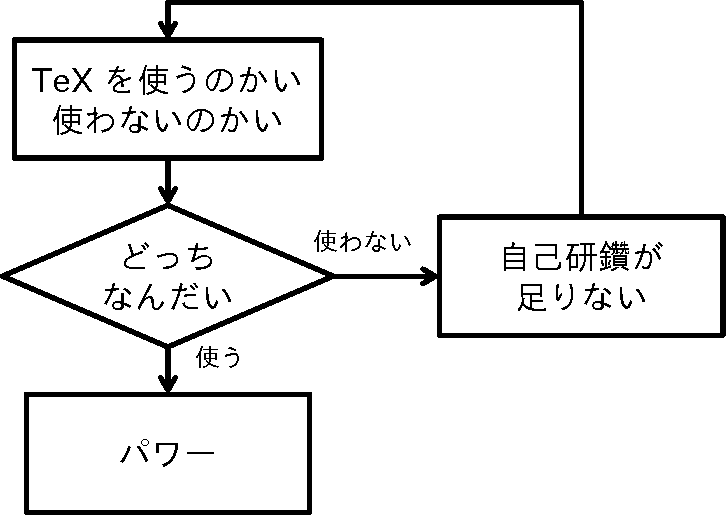
\includegraphics[width=0.8\linewidth]{./figures/power.pdf}
    \caption{ベクタ形式}
    \label{fig:ベクタ形式}
  \end{subfigure}
  \hfill
  \begin{subfigure}{\myLineWidth}
    \centering
    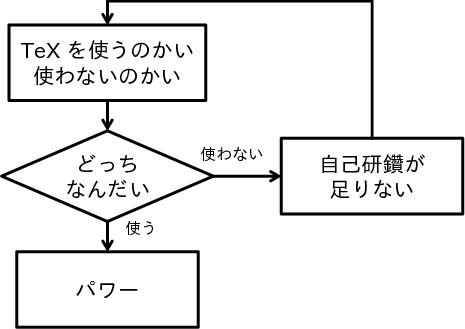
\includegraphics[width=0.8\linewidth]{./figures/power.png}
    \caption{ラスタ形式}
    \label{fig:ラスタ形式}
  \end{subfigure}
  \caption{図の比較}
\end{figure*}

\subsubsection{高度な数式}
\label{sec:高度な数式}

\verb|mathtools|パッケージを用いることで，
より高度な数式を記述できます．
\verb|mathtools|パッケージは，
\verb|amsmath|パッケージを内部で読み込みます．
このパッケージを用いる場合，
これを\verb|newtx|パッケージよりも\emph{前に}指定してください．

\verb|bm|パッケージを用いることで，
数式中で$\bm{v}$や$\bm{M}$などの太字を簡単に表示できます．
$\bm{\alpha}$や$\bm{\beta}$などのギリシャ文字も太字にできます．
このパッケージを用いる場合，
これを\verb|newtx|パッケージよりも\emph{後に}指定してください．

\subsection{図表}

図や表を配置するために，
\verb|figure|環境や\verb|table|環境を用います．
二段抜きの場合は，
\verb|figure*|\+環境や\verb|table*|\+環境を用います．
\verb|[t]|や\verb|[tb]|のように，
出力位置を指定するためのオプションを\emph{必ず}指定してください．

\subsubsection{画像の取り込み}

\verb|graphicx|パッケージを用いることで，
画像の取り込みを行えます．
ブロック図やグラフなど，
線による描画が主である画像を取り込む場合，
PDFやEPSなどのベクタ形式の使用を検討してください．
ベクタ形式の図は拡大してもボヤけずに表示できます．
\図{fig:ベクタ形式}と\図{fig:ラスタ形式}とを比較してください．
図を取り込む際，
\verb|width=\linewidth|のオプションを指定すると，
行の幅一杯に画像を表示できます．
\文献{美文書}の第7章を併せて参照してください．

\verb|pdfcrop|コマンドを用いることで，
PDFファイルの余白を削除できます．
このコマンドは，{\TeX} Liveに含まれています．
例えば，次のように実行すると，
\texttt{file.pdf}の余白を削除した\texttt{file-crop.pdf}が生成されます．

\begin{uitexconsole}
pdfcrop file.pdf
\end{uitexconsole}

\begin{thebibliography}{9}
  \bibitem{TeXWiki}
    \enquote{{\TeX} Wiki},
    <\url{https://texwiki.texjp.org/}>,
    accessed in 2026-09.
  \bibitem{美文書}
    奥村晴彦，黒木裕介：
    「［改訂第9版］{\LaTeX}美文書作成入門」，
    株式会社技術評論社，
    東京
    （2023）．
  \bibitem{PTUForum}
    職業能力開発総合大学校：
    「PTUフォーラム」，
    基盤整備センター，
    <\url{https://www.uitec.jeed.go.jp/kiban/research/}>，
    2026-09参照．
  \bibitem{uitex}
    KusaReMKN:
    \enquote{KusaReMKN/uitex},
    GitHub,
    <\url{https://github.com/KusaReMKN/uitex}>,
    accessed in 2026-09.
  \bibitem{jlreq}
    N.~Abe:
    \enquote{abenori/jlreq},
    GitHub,
    <\url{https://github.com/abenori/jlreq}>,
    accessed in 2026-09.

\end{thebibliography}

\section{クラスファイルの説明}

クラスファイル\texttt{uitex.cls}は，
職業能力開発研究発表会の講演論文のための体裁を提供します．
GitHub（\url{https://github.com/KusaReMKN/uitex}）から
このクラスファイルの最新版をダウンロードできます．
なお，このクラスファイルは\texttt{jlreq}をラップしたものです\Cite{jlreq}．

\subsection{テンプレートと記述方法}

\図{fig:記述例}のように記述します．
このクラスファイルに同梱される
ファイル\texttt{template.tex}も参照してください．
\begin{figure}[t]
  \small\hrulefill% 見栄えのため
\begin{verbatim*}
\documentclass[lualatex,fleqn]{uitex}
%\usepackage{graphicx}% 図の取り込み
\usepackage{mathtools,amssymb}% 数式関連
\usepackage[varg]{newtx}% 英数フォント
\usepackage{mknmacro}% 便利マクロ集
\title{論文タイトル\\改行もできます}
\author{%
  ○能開 花子，教育 一郎（某大学校），
  研究 二郎（職業未来技研），\\% 改行できます
  発明 三郎（ものづくり製作所）}
\pagestyle{forum}% 講演論文の体裁
\ForumNumber{36}% 第何回
\ForumDate{2026/11/27〜28}% 開催日
\begin{document}
\maketitle
\section{はじめに}
ほげほげ……
\begin{thebibliography}{9}
  \bibitem{}
\end{thebibliography}
\end{document}
\end{verbatim*}
\hrulefill
  \caption{記述例}
  \label{fig:記述例}
\end{figure}

記述すべき項目について順に説明します．

\begin{itemize}
  \item
    クラスオプションに\texttt{lualatex}や\texttt{uplatex,dvipdfmx}など，
    組版に用いるエンジンを指定してください．
    できれば，(u)\pLaTeX よりもLua\LaTeX を積極的に用いるようにしてください．
  \item
    Times系のフォントを利用するため，\texttt{newtx}パッケージを用います．
    例には記述されていませんが，
    和文フォントの見た目が雅びすぎるように思われる場合，
    IPAexフォントを利用することで
    MSフォントの風合いに近付けられるかもしれません．
  \item
    スタイルファイル\texttt{mknmacro.sty}を用いる場合は記述します．
    詳細は\ref{sec:mknmacro}を参照してください．
  \item
    \verb|\title|で論文タイトルを指定します．
    タイトル中で改行するには \verb|\\| を用います．
  \item
    \verb|\author|で著者を指定します．
    各著者を全角カンマ（，）で区切ります．
    所属は全角丸括弧「（」「）」で囲んで表示します．
    やはり \verb|\\| で改行できます．
  \item
    \verb|\pagestyle|で体裁を指定します．
    \texttt{forum}を指定してこの体裁にします．
  \item
    \verb|\ForumNumber|，及び \verb|\ForumDate|で
    PTUフォーラムの開催される回，及び日付をそれぞれ指定します．
  \item
    \verb|\maketitle|で論文タイトルと著者一覧とが出力されます．
\end{itemize}

\subsection{見出し}

見出しが連続する
（\verb|\section|の直後に \verb|\subsection|が続くなど）場合，
適切な行取りとなるように設定されています
（「論文テンプレート」の3.と3.1.との間や3.4.と3.4.1.との間と同様になります）．

\subsection{数式}

ディスプレイ数式は\式{eq:数式例}のように表示されます．
数式を参照するために \verb|\eqref|を使うと便利です．
\begin{equation}
  \zeta(s)
  \coloneq \sum_{n=1}^{\infty} \frac{1}{n^s}
  = \frac{1}{1^s} + \frac{1}{2^s} + \frac{1}{3^s} + \frac{1}{4^s} + \cdots
  \label{eq:数式例}
\end{equation}

\subsubsection{より高度な数式}

より高度な数式の記述のために\texttt{mathtools}パッケージを使えます
（\texttt{mathtools}パッケージは\texttt{amsmath}パッケージを内部で用います）．
このパッケージを用いる場合，\texttt{newtx}パッケージより先に指定してください．

また，太字（$\bm{v}$や$\bm{M}$など）のために\texttt{bm}パッケージを用いる場合，
\texttt{newtx}パッケージより後に指定してください．

\subsection{図表}

図や表を配置するために
\texttt{figure}環境や\texttt{table}環境を用いてください．
二段抜きの場合は\texttt{figure*} 環境や\texttt{table*} 環境を用います．
出力位置を指定するためのオプション
（\texttt{[t]}や\texttt{[tb]}など）を必ず指定してください．

\subsubsection{図の取り込み}

図を取り込むために\texttt{graphicx}パッケージを用います．
\begin{verbatim}\usepackage{graphicx}\end{verbatim}

ブロック図やグラフなどを取り込む場合，
PDFやEPSなどのベクタ形式を用いることを検討してください．
ベクタ形式の図は拡大してもボヤけずに表示できます．
\図{fig:vector}と\図{fig:raster}とを比較してください．
\begin{figure}[tb]
  \centering
  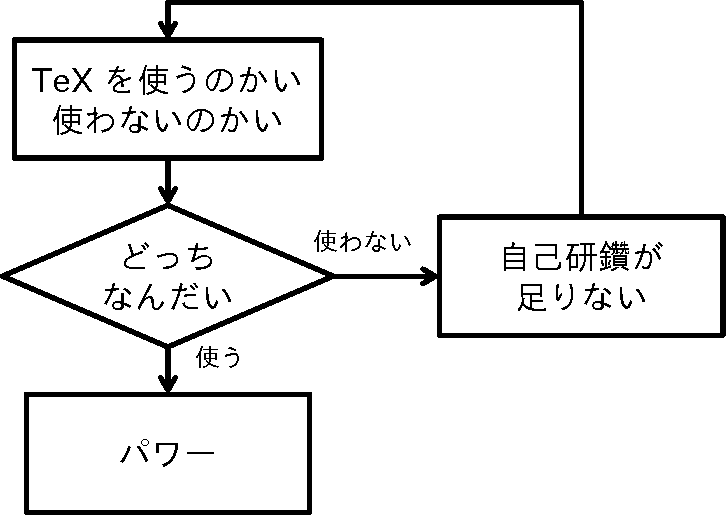
\includegraphics[width=0.8\linewidth]{./figures/power.pdf}
  \caption{ベクタ形式}
  \label{fig:vector}
\end{figure}
\begin{figure}[tb]
  \centering
  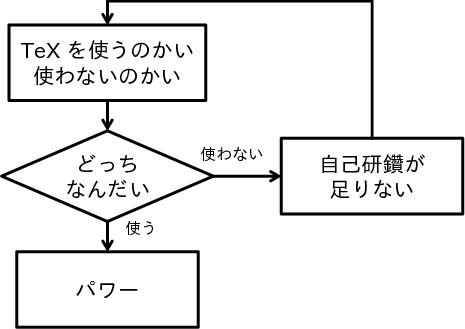
\includegraphics[width=0.8\linewidth]{./figures/power.png}
  \caption{ラスタ形式}
  \label{fig:raster}
\end{figure}

\texttt{pdfcrop}コマンドを用いてPDFファイルの余白を削除できます．
このコマンドは\TeX\ Liveに含まれています．
\begin{verbatim}$ pdfcrop file.pdf\end{verbatim}

図を取り込む際，
\verb|width=\linewidth|を指定して行の幅一杯に画像を表示できます．
\begin{verbatim}\includegraphics[width=\linewidth]{file.pdf}\end{verbatim}

\文献{奥村}の第7章もまた参照してください．

\subsubsection{表の記述}

表は少し小さい文字（\verb|\small|）で組まれます．
\図{fig:表の例}のように記述すると\表{tab:表の例}が得られます．
表の一番上と一番下の罫線を太くするために，\verb|\Hline|を用いてください．
また，\文献{奥村}の第8章も参照してください．
\begin{figure}[tb]
  \small\hrulefill% 見栄えのため
\begin{verbatim}
\begin{table}[tb]
  \centering
  \caption{イロイロな個性}
  \label{tab:表の例}
  \begin{tabular}{cc}
    \Hline
    外観 & 特徴 \\
    \hline
    赤色 & 火に強い \\
    青色 & 溺れない \\
    黄色 & 高く飛ぶ \\
    紫色 & 力持ち \\
    白色 & 毒がある \\
    \Hline
  \end{tabular}
\end{table}
\end{verbatim}
  \hrulefill
  \caption{表の記述例}
  \label{fig:表の例}
\end{figure}
\begin{table}[tb]
  \centering
  \caption{イロイロな個性}
  \label{tab:表の例}
  \begin{tabular}{cc}
    \Hline
    外観 & 特徴 \\
    \hline
    赤色 & 火に強い \\
    青色 & 溺れない \\
    黄色 & 高く飛ぶ \\
    紫色 & 力持ち \\
    白色 & 毒がある \\
    \Hline
  \end{tabular}
\end{table}

\subsection{参考文献}

参考文献における文献リストの記述が特殊であるため，
\BibTeX を使うことは推奨できません．
手動で\texttt{thebibliography}環境を入力してください．

文献引用を引用するための \verb|\cite|は通常の（上付きでない）引用です．
上付きの引用は \verb|\Cite|を用います．
「\verb|文献\cite{奥村}|」は「文献\cite{奥村}」のように，
\verb|\Cite{奥村}| は文末のようになります\Cite{奥村}．

\subsection{注釈}

脚注を使えます
\footnote{脚注はこのように表示されます．}．
実は割注\warichu{こんな感じに挿入される注}も使えます．
詳細については\文献{jlreq}も参照してください．

\section{記述する上での注意}

和文中の句読点や括弧類は，全角のもの（，）（．）「（」「）」を用いてください．
半角のもの（,）（.）「(」「)」を用いると幅や高さが合わなくなり，
不恰好に見えます．
特に，参考文献リストにおける和文の項目については，
全角のコロンやカンマ，ピリオドを用いてください．
欧文中の句読点や括弧類は，半角のものを用いてください．

ハイフンとダーシを使い分けてください．
ハイフン（\verb|-|）は，主に二つの単語を接続する用途で用います
（well-knownなど）．
二分ダーシ（\verb|--|）は，主に範囲を表す用途で用います
（pp.29--57など）．

改行（\verb|\\|）を濫用しないでください．
ただし，あなたが詩を書いている場合，この限りではありません．
同時に\texttt{verse}環境の併用を検討してください．

国際単位系を用いる場合には\texttt{siunitx}パッケージが便利です．
例えば，「\verb|\qty{1}{\milli\metre}|」で
「\qty{1}{\milli\metre}」のようになります．
詳細は\texttt{siunitx}パッケージのドキュメントを参照してください．
\begin{verbatim}$ texdoc siunitx\end{verbatim}

URLを記述する場合には\texttt{url}パッケージが便利です．
例えば，「\verb|\url{https://example.com/}|」は
「\url{https://example.com/}」のようになります．
メールアドレスを記述する場合も同様です．
詳細は\texttt{url}パッケージのドキュメントを参照してください．
\begin{verbatim}$ texdoc url\end{verbatim}

\section{追加のマクロ}
\label{sec:mknmacro}

クラスファイル\texttt{uitex.cls}に加え，
スタイルファイル\texttt{mknmacro.sty}を同梱しています．
このファイルには，いくつかの便利なマクロを収録しています．

\subsection{括弧}

数式中で用いる括弧類のマクロを定義しています．
これらのマクロのために，\texttt{mathtools}パッケージを利用しています．
「\verb|a+\bq{b+\brq{c+\pq{d+e}}}|」は
「$a+\bq{b+\brq{c+\pq{d+e}}}$」のようになります．
これらのマクロは括弧の中身が大きくなる際に真価を発揮します．
星付き命令（\verb|\pq*| など）を用いることで，
括弧の中身に応じて自動的に括弧のサイズを調整します．
\verb|y = \pq*{\frac{x+1}{x}}^{x}| で\式{eq:括弧例}を得られます．
\begin{equation}
  y
  = \pq*{\frac{x+1}{x}}^{x}
  \label{eq:括弧例}
\end{equation}

同様に，絶対値（\verb|\abs|）や床関数（\verb|\floor|），
天井関数（\verb|\ceil|）も用意しています（\式{eq:括弧例2}）．
\begin{equation}
  \ceil*{\frac{\vphantom{1}a}{b}}
  = \floor*{\frac{a+b-1}{b}}
  = \floor*{\frac{a-1}{b}}+1
  \label{eq:括弧例2}
\end{equation}

\subsection{参照}

参照を表示するためのマクロ
（\verb|\図|，\verb|\表|，\verb|\式|，及び\break\verb|\文献|）を
定義しています．
「\verb|\表{tab:表の例}|」は
「\表{tab:表の例}」のようになります．
波括弧の中には \verb|\ref|や \verb|\cite|で指定するものを指定します．
「表1」の「表」と「1」との間で改行されてしまうと不格好ですから，
これらを抑制するように設定してあります．


\begin{thebibliography}{9}
  \bibitem{AMAMOGU}
    iON!：
    「バチモリーナ」，
    YouTube，
    \url{https://www.youtube.com/watch?v=BbmIQocY6Iw}
    （2025）．
  \bibitem{jlreq}
    Abe, N., and contributors:
    ``abenori/jlreq'',
    GitHub,
    \url{https://github.com/abenori/jlreq}
    (2025).
  \bibitem{奥村}
    奥村晴彦，黒木裕介：
    「［改訂第9版］\LaTeX 美文書作成入門」，
    技術評論社，
    東京
    （2023）．
\end{thebibliography}

\end{document}
% mkn: forceComma forcePeriod :
% ex: se et ts=2 :
